\section{ТЕХНОЛОГИЧЕСКИЙ РАЗДЕЛ}

\subsection{Описание аппаратной платформы для приема сигналов GPS}
Аппаратная платформа подразделяется на несколько частей: RF-часть, память, интерфейс управления и передачи данных, ПЛИС-микросхема
на которой реализованы все контроллеры и интерфейсы, а также вся управляющая логика платы. Схемы тракта передачи данных
представлена на рисунке \ref{pic:board_scheme}. Данные поступают с антенны на МШУ, потом проходят в ширикополосный фильтр, далее
данные записываются на SRAM-микросхему памяти и передаются через интерфейс RS-232 на комьютер. ПО управления платой имеет механизм
дальнейшей публикации дампа данных в любое хранилище данных (ftp, www, samba, nfs и т.д.). 

\begin{figure}[H]
\center{\includegraphics[width=1\linewidth]{./pics/main_tract.eps}}
\caption{Система захвата данных - тракт данных}
\label{pic:board_scheme}
\end{figure}

Компонентами на плате управляет ПЛИС-микросхема. На основе этой микросхемы были разработаны: контроллер памяти (раздел \ref{sec:sram_controller}), реализация RS-232
интерфейса (раздел \ref{sec:rs232}), последовательный интерфейс программирования MAX2769 (раздел \ref{sec:gps_program}), модуль захвата данных
(раздел \ref{sec:gps_acq}), а также вспомогательные модули. В рабочем режиме плата ждет команд с RS-232 интерфейса. Команды выдает
управляющее ПО (board daemon) - сервис разработанный под ОС Linux (раздел \ref{sec:board_daemon}). 

\begin{figure}[H]
\begin{center}
	\scalebox{0.5}{\includegraphics[width=1\linewidth]{./pics/fpga_scheme.eps}}
\end{center}
\caption{Система захвата данных - ПЛИС архитектура}
\label{pic:fpga_scheme}
\end{figure}

На рисунке \ref{pic:fpga_scheme} представлена схема взаимодествия модулей. Модуль top\_level объединяет все внешние модули и 
управляет мультиплексированием внешних сигналов.

%=====================================================================
\subsection{Описание разработанных встраиваемых решений (VHDL)}
\subsubsection*{Арбитр GPS-Board}
Арбитр платы выполняет основную управляющую функцию. Внутри арбитра происходит разбор пришедших по RS-232 команд, определяется
модуль, который будет управлять SRAM, осуществляется координация действий всех остальных модулей. Архитектура модуля представлена на
рисунке \ref{pic:arbiter_arch}.

\begin{figure}[h]
\begin{center}
	\scalebox{0.3}{\includegraphics[width=1\linewidth]{./pics/arbiter_arch.eps}}
\end{center}
\caption{Арбитр GPS-Board}
\label{pic:arbiter_arch}
\end{figure}

Сигнал mode[1:0] управляет мультиплексором, который определяет модуль, получающий доступ к SRAM. 

Так же арбитер управляет записью в SRAM клиентских данных и выдачей содержимого SRAM через RS-232 клиенту. Для этого используются
сигналы rw, mem, data\_f2s[7:0], data\_s2f[7:0], addr\_a[17:0]. Арбитр устанавливает сигнал mode[1:0] в соостояние соответствующее
тому, что он управляет SRAM и начинает цикл чтения/записи. После получения сигнала ready цикл чтения/записи считается завершенным
и данные записанными/валидными.

Модуль захвата GNSS сигнала управляется сигналом gps\_start\_a.
При получении команды по RS-232 на захват данных, сигнал gps\_start\_a выставляется
и арбитер переходит в режим ожидания сигнала gps\_done\_a, символизирующего окончания захвата (заполнение микросхемы памяти).
Арбитр, получив данный сигнал, отправляет ответ по RS-232 об успешном захвате.

Сигналы cs\_a, sclk\_a, sdata\_a используются для программирования микросхемы MAX2769. Модуль программирования данной микросхемы
описан внутри модуля арбитра, поэтому все сигналы управления являются внутренними относительно арбитра и не представлены на рисунке
\ref{pic:arbiter_arch}. 

Сигнал test\_mem управляет модуль тестирования памяти. Получив команду тестирования, арбитр переходит в режим ожидания окончания теста.
Двух битная шина test\_result[1:0] возвращает результат тестирования в арбитр. Арбитр анализирует ответ и возвращает результат 
через RS-232 интерфейс клиенту.

Программирование режимов GPS микросхемы происходит через последовательный порт. Временные критерии и их значения
отражены на таблице ~\ref{tab:gps_serial}.

%\begin{figure}[h]
%\center{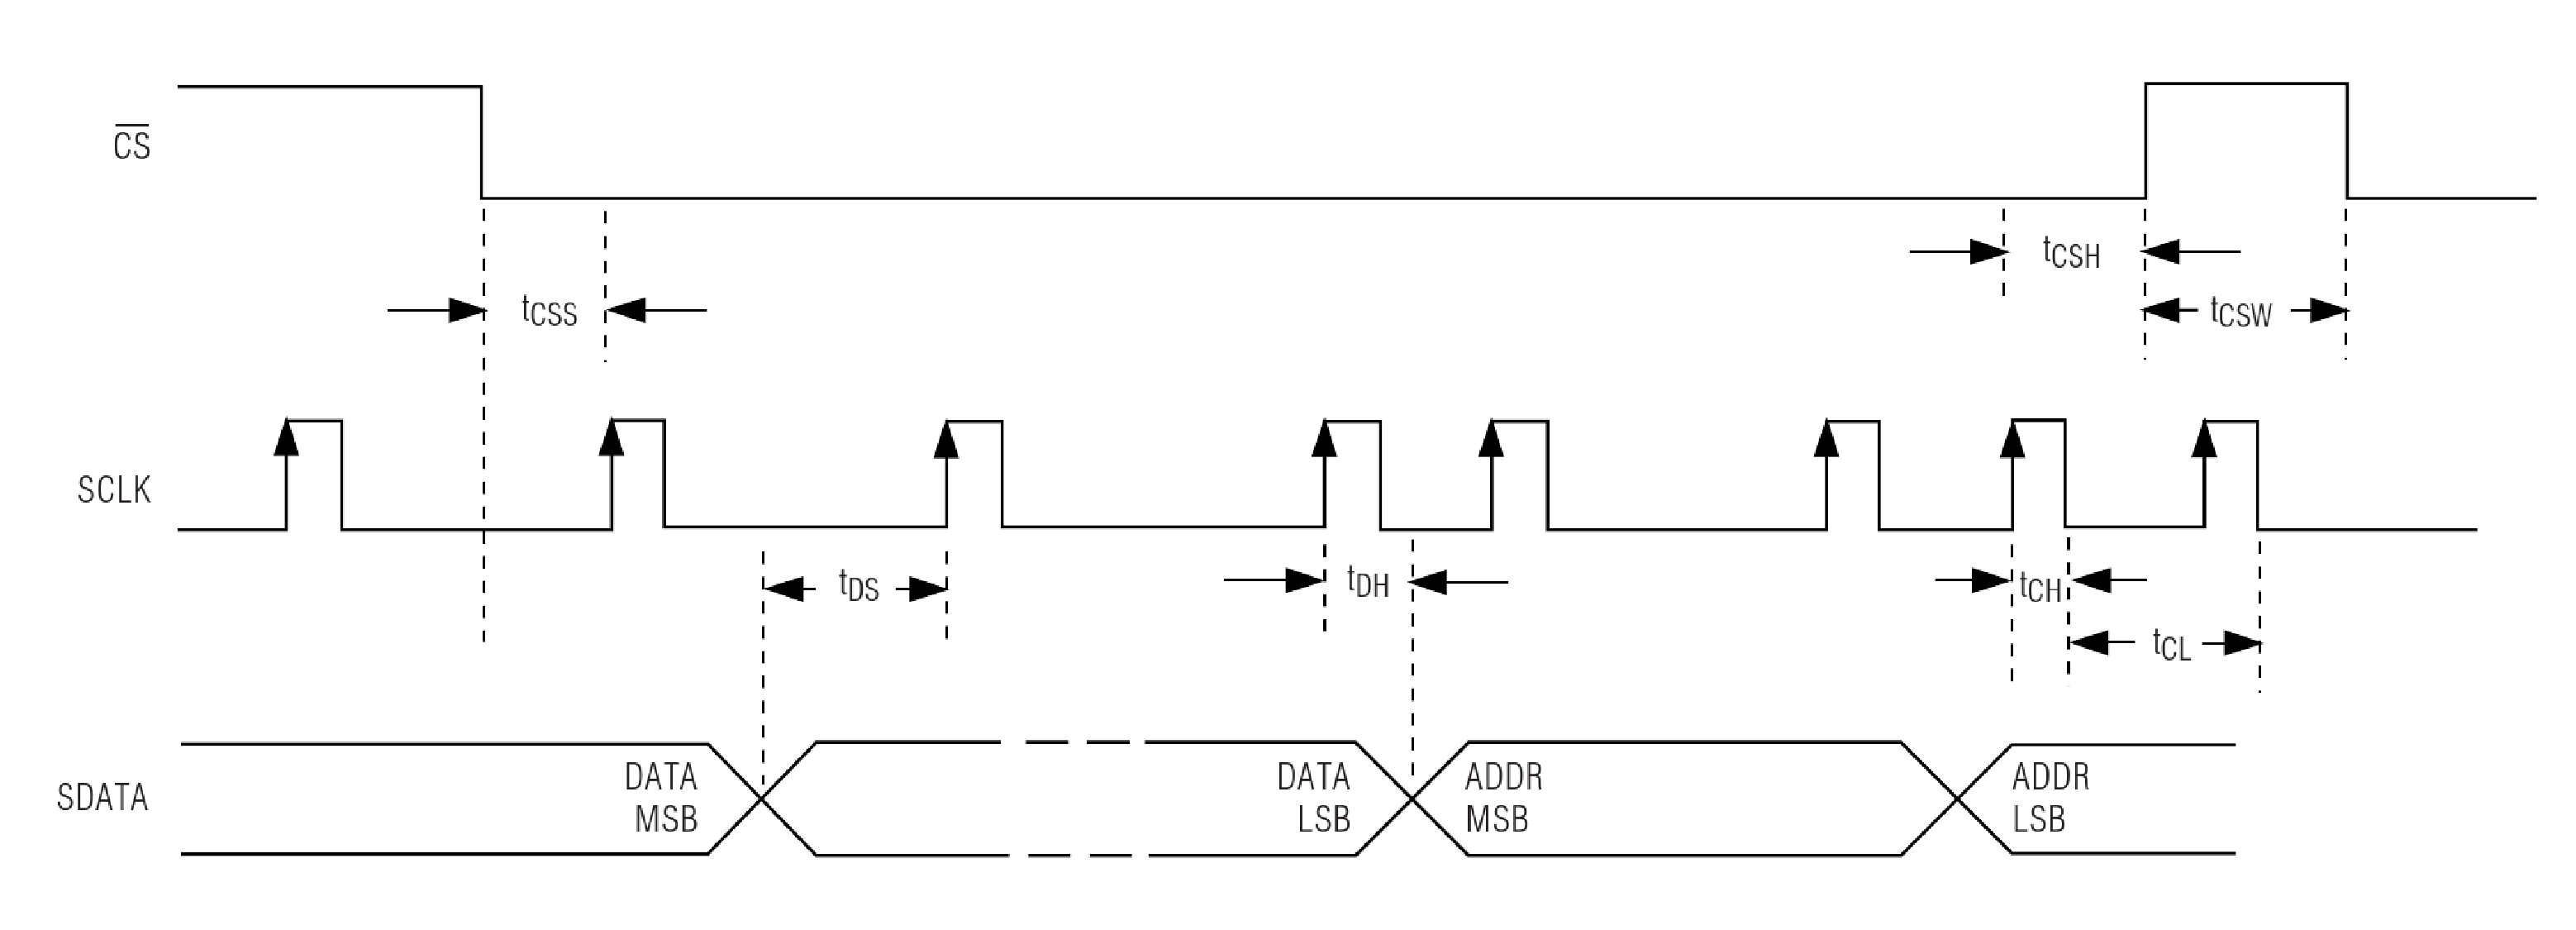
\includegraphics[width=1\linewidth]{./pics/gps_serial_times.eps}}
%\caption{Временная диарамма serial-интерфейса GPS}
%\label{pic:gps_serial}
%\end{figure}

\begin{table}[h]
\caption{Временные требования для serial-интерфейса}
\label{tab:gps_serial}
\begin{tabular}{|c|p{250pt}|c|p{70pt}|}
 \hline  
  Символ & Параметр & Значение & Единица измерения  \\  
 \hline  
  $t_{css}$  & Время между падающим фронтом сигнала $\bar {CS}$ и передним фронтом сигнала SCLK	& 10 & нс  \\  
 \hline  
  $t_{ds}$   & Время установки данных на serial-линию	& 10 & нс \\  
 \hline  
  $t_{dh}$   & Время удержания данных на serial-линии	& 10 & нс \\  
 \hline  
  $t_{ch}$   & Время нахождения Сlock-сигнала serial-интерфейса в состоянии 1 & 25 & нс \\  
 \hline  
  $t_{cl}$   & Время нахождения Сlock-сигнала serial-интерфейса в состоянии 0 & 25 & нс \\  
 \hline  
  $t_{csh}$  & Время между крайним возрастающим фронтом сигнала SCLK и падающим фронтом сигнала $\bar {CS}$ & 10 & нс \\  
 \hline  
  $t_{csw}$  & Время $\bar {CS}$ в активном состоянии    & 1 & такт \\  
 \hline  
\end{tabular}
\end{table}

Значения регистров можно найти в руководстве на микросхему MAX2769.

\subsubsection*{RS-232}
\label{sec:rs232}
RS232 интерфейс является последовательным портом. Существует несколько режимов работы данного порта, но я рассмотрю только один
из них - режим с одним стартовым и одним стоповым битом без контроля передачи данных. На рисунке \ref{pic:rs232_wire} представлен
цикл передачи 0x55 значения по данному интерфейсу. В режиме ожидания (IDLE-режим) напряжение на линии TX-RX -10В (или между -5В и -15В).
При поступлении нулевого бита (стартовый бит - начало транзакции) на линии устанавливается напряжение +10В (или между +5В и +15В).
После передачи 8 битов данных, транзакцию завершает 1 стоповой бит - единичный бит.

\begin{figure}[H]
\center{\includegraphics[width=1\linewidth]{./pics/rs232_wire.eps}}
\caption{RS232 интерфейс}
\label{pic:rs232_wire}
\end{figure}

Для реализации интерфейса RS232 на данной плате необходимо разработать делитель частоты, так как самым быстрым режимом передачи данных
для RS-232 порта является скороть 115200 б/c. Так же необходимо реализовать прием команд длинной 64 бита, чтобы обеспечить
полный функционал (программирование GPS-микросхемы, запись в память, управление платой).

\subsubsection*{Контроллер для SRAM-микросхемы M5M5V208FP-85}
\label{sec:sram_controller}
Рабочий режим M5M5V208 определяется комбинацией управляющих сигналов устройства $\bar{S_1}$, ${S_2}$, $\bar{W}$ и $\bar{OE}$.
Цикл чтения выполняется при низком уровне $\bar{W}$, перекрываемом низким уровнем $\bar{S_1}$ и высоким уровнем ${S_2}$.
Подробнее последовательность действий отражена на Рис.~\ref{pic:sram_write_cycle} и Таблице~\ref{tab:sram_write_cycle},
техническая релизация рассмотрена в разделе~\ref{sec:sram_controller}.

\begin{figure}[H]
\center{\scalebox{0.8}{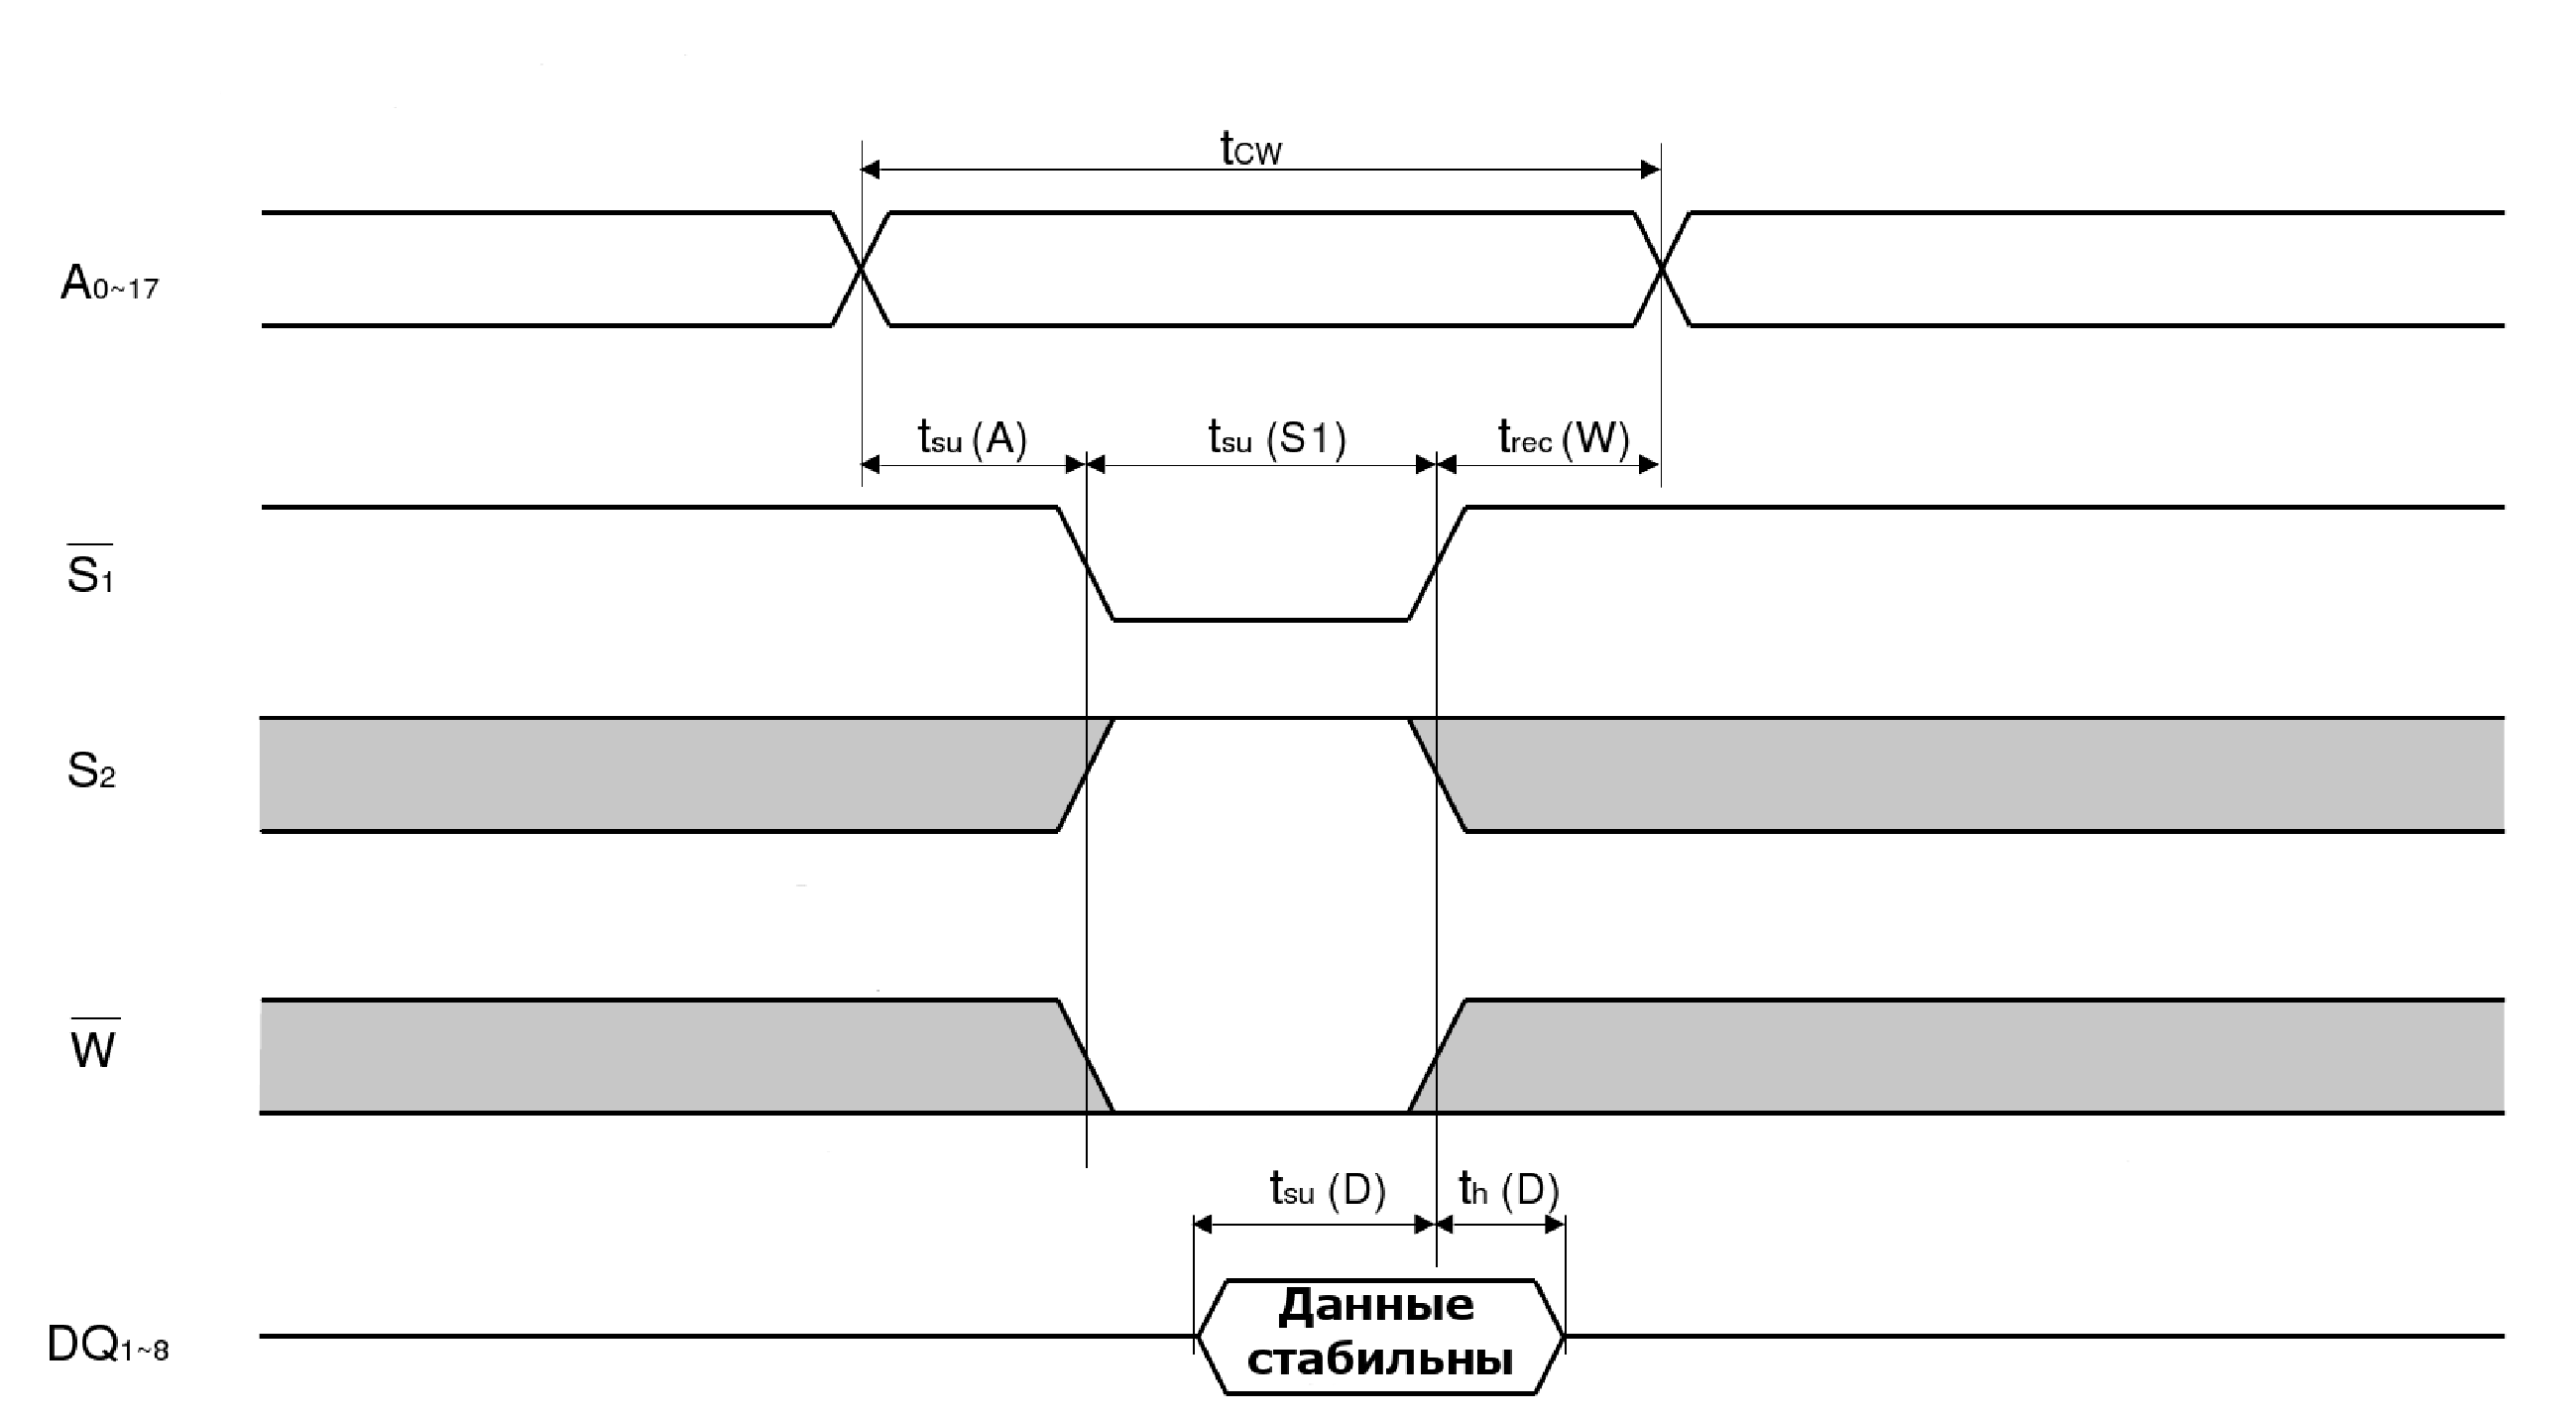
\includegraphics[width=1\linewidth]{./pics/sram_write_cycle.eps} }}
\caption{Цикл записи}
\label{pic:sram_write_cycle}
\end{figure}

\begin{center}
\begin{longtable}{|c|p{7cm}|c|c|}
\caption{Цикл операции чтения из SRAM} \label{tab:sram_write_cycle} \\ \hline
\multicolumn{1}{|p{3cm}|}{\textbf{Название цикла}}    &   \multicolumn{1}{c|}{\textbf{Обозначение}} & 
\multicolumn{1}{|c|}{\textbf{Время}}    &   \multicolumn{1}{c|}{\textbf{Единицы}} \\ \hline

\multicolumn{1}{|c|}{\textbf{1}}    &   \multicolumn{1}{|c|}{\textbf{2}} &
\multicolumn{1}{|c|}{\textbf{3}}    &   \multicolumn{1}{|c|}{\textbf{4}} \\ \hline
\endfirsthead

\multicolumn{2}{|l|}{{Продолжение таблицы ~\ref{tab:sram_read_cycle}}} \\ %\hline
\hline
\multicolumn{1}{|c|}{\textbf{1}}    &   \multicolumn{1}{|c|}{\textbf{2}} &
\multicolumn{1}{|c|}{\textbf{3}}    &   \multicolumn{1}{|c|}{\textbf{4}} \\ \hline
\endhead
\endfoot

	\hline
		Название цикла & Обозначение & Время & Единицы \\
	\hline
		${t_{cw}}$ & Время цикла записи & 85 & ns \\
	\hline
		${t_w(W)}$ & Вркмя пульса записи & 60 & ns \\
	\hline
		${t_{su}(A)}$ & Время установки адреса & 0 & ns \\
	\hline
		${t_{su}(A-WH)}$ & Время установки адреса в соотв. с $\bar{E}$ & 70 & ns \\
	\hline
		${t_{su}(S_1)}$ & Время установки Chip Select 1 & 70 & ns \\
	\hline
		${t_{su}(S_2)}$ & Время установки Chip Select 1 & 70 & ns \\
	\hline
		${t_{su}(D)}$ & Время установки данных & 35 & ns \\
	\hline
		${t_{h}(D)}$ & Время удержания данных & 0 & ns \\
	\hline
		${t_{rec}(W)}$ & Время восстановления & 0 & ns \\
	\hline
		${t_{dis}(W)}$ & Время перехода после $\bar{W}$ низкого & 30 & ns \\
	\hline
		${t_{dis}(OE)}$ & Время перехода после $\bar{OE}$ высокого & 30 & ns \\
	\hline
		${t_{en}(W)}$ & Время перехода после $\bar{W}$ высокого & 30 & ns \\
	\hline
		${t_{en}(OE)}$ & Время перехода после $\bar{OE}$ низкого & 30 & ns \\
	\hline
\end{longtable}
\end{center}

Цикл чтения выполняется при высоком уровне сигнала $\bar{W}$ и низком уровне сигнала OE. В то же время сигналы
$\bar{S_1}$ и ${S_2}$ должны находится в активном состоянии. 

\begin{figure}[h]
\center{\scalebox{0.8}{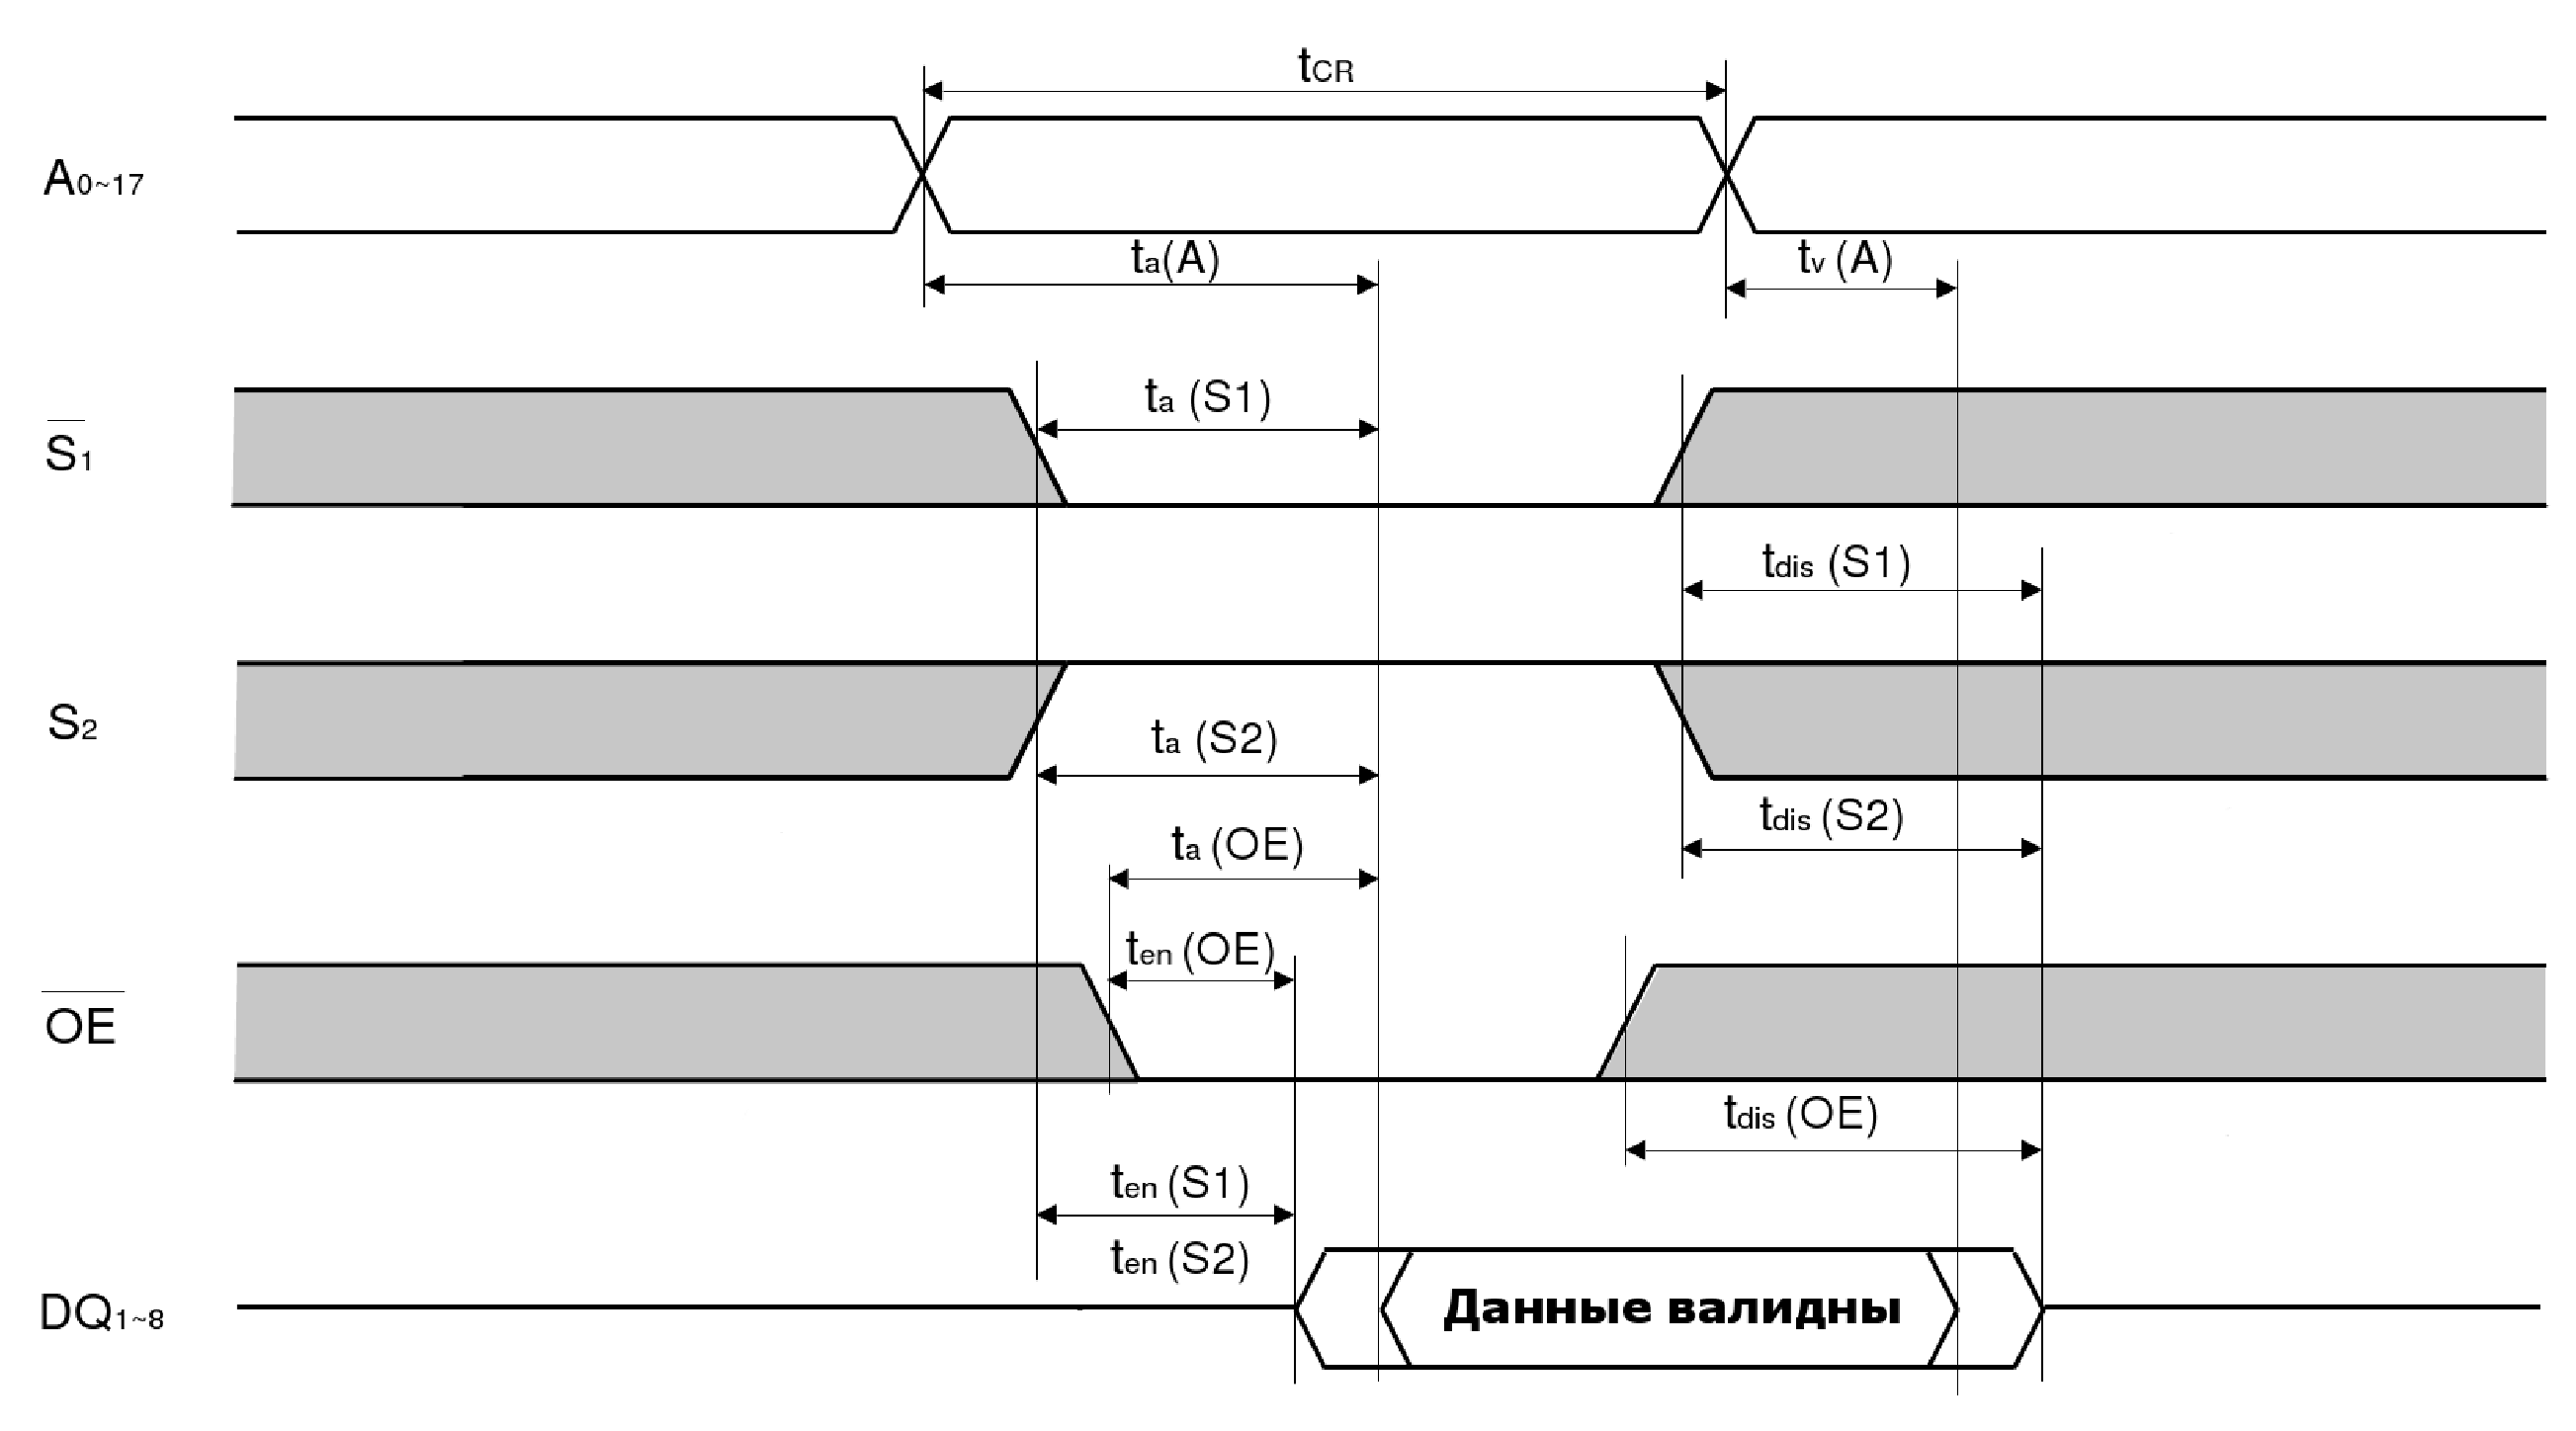
\includegraphics[width=1\linewidth]{./pics/sram_read_cycle.eps}}}
\caption{Цикл чтения}
\label{pic:sram_read_cycle}
\end{figure}

\begin{center}
\begin{longtable}{|c|p{7cm}|c|c|}
\caption{Цикл операции чтения из SRAM} \label{tab:sram_read_cycle} \\ \hline
\multicolumn{1}{|p{3cm}|}{\textbf{Название цикла}}    &   \multicolumn{1}{c|}{\textbf{Обозначение}} & 
\multicolumn{1}{|c|}{\textbf{Время}}    &   \multicolumn{1}{c|}{\textbf{Единицы}} \\ \hline

\multicolumn{1}{|c|}{\textbf{1}}    &   \multicolumn{1}{|c|}{\textbf{2}} &
\multicolumn{1}{|c|}{\textbf{3}}    &   \multicolumn{1}{|c|}{\textbf{4}} \\ \hline
\endfirsthead

\multicolumn{2}{|l|}{{Продолжение таблицы ~\ref{tab:sram_read_cycle}}} \\ %\hline
\hline
\multicolumn{1}{|c|}{\textbf{1}}    &   \multicolumn{1}{|c|}{\textbf{2}} &
\multicolumn{1}{|c|}{\textbf{3}}    &   \multicolumn{1}{|c|}{\textbf{4}} \\ \hline
\endhead
\endfoot

	\hline
		 &  &  &  \\
	\hline
		${t_{cr}(A)}$ & Время цикла чтения & 85 & ns \\
	\hline
		${t_a(A)}$ & Время доступа к адресу & 85 & ns \\
	\hline
		${t_a(S_1)}$ & Chip Select 1 & 85 & ns \\
	\hline
		${t_a(S_1)}$ & Chip Select 2 & 85 & ns \\
	\hline
		${t_a(OE)}$ & Время доступа к активному уровню OE & 45 & ns \\
	\hline
		${t_{dis}(S_1)}$ & Время перехода к низкому уровню & 30 & ns \\
	\hline
		${t_{dis}(S_2)}$ & Время перехода к низкому уровню & 30 & ns \\
	\hline
		${t_{dis}(OE)}$ & Время перехода после $\bar{OE}$ высокого уровня & 30 & ns \\
	\hline
		${t_{en}(S_1)}$ & Переход к активному состоянию для $\bar{S_1}$ & 10 & ns \\
	\hline
		${t_{en}(S_1)}$ & Переход к активному состоянию для ${S_2}$ & 10 & ns \\
	\hline
		${t_{en}(OE)}$ & Переход к активному состоянию для $\bar{OE}$ & 5 & ns \\
	\hline
		${t_{v}(A)}$ & Время валидности данных $\bar{OE}$ & 10 & ns \\
	\hline

\end{longtable}
\end{center}

Полное описание работы данной SRAM-микросхемы памяти приводится в описании на микросхему M5M5V208FP-85.

Контроллер микросхемы памяти был реализован на VHDL. Структурная схема представлена на рисунке \ref{pic:sram_arch}.

\begin{figure}[H]
\begin{center}
	\scalebox{0.5}{\includegraphics[width=1\linewidth]{./pics/sram_arch.eps}}
\end{center}
\caption{Контроллер SRAM-памяти}
\label{pic:sram_arch}
\end{figure}

Входной сигнал rw управляет режимами чтения/записи, преобразую заданный режим в комбинацию выходных сигналов OE, WE, s1, s2.
Шина data\_f2s[7:0] является входной шиной, через нее модули записывают данные в SRAM. Внутри модуля байт из data\_f2s
переносится в локальный сигнал и выставляется на запись в шину dio\_a[7:0]. Шина data\_f2s[7:0] мультиплексная, потому что 
у памяти есть несколько клиентов: модуль тестирования памяти, арбитр, модуль захвата сигналов GNSS. Сигнал mem сигнализирует о начале
активности. Так же мультиплексируются все сигналы задействованные при записи данных в SRAM: rw, mem\_s, addr[17:0]. Сигналом окончания
цикла чтения/записи является сигнал ready.

\subsubsection*{Модуль тестирования SRAM-микросхемы M5M5V208FP-85}
\label{sec:test_sram}
Модуль тестирования реализует просто тест памяти по методике бегущего бита (walking bit). Поскольку объем памяти невелик, а скорость
достаточно высокая, возможно протестировать данным тестом всю микросхему. Суть теста заключается в том, что в каждый адрес записывается
байт всего с одной единицей, в следующий за данным адресом записывается байт со сдвинутой единицей на 1 разряд. При перенесении единицы
из 7 разряда, она вносится в 0-ой разряд. Модуль сначала записывает бегущую единицу во все ячейки, а потом считывает и сравнивает с
копией бегущей единицы. Данный тест позволяет детектировать практически все виды ошибок памяти:
разрыв дорожки, замыкание дорожек, отсутствие чипа, нарушение работы чипа. Архитектура модуля представлена на рисунке
\ref{pic:test_sram_arch}.

\begin{figure}[h]
\begin{center}
	\scalebox{0.4}{\includegraphics[width=1\linewidth]{./pics/test_sram_arch.eps}}
\end{center}
\caption{Контроллер SRAM-памяти}
\label{pic:test_sram_arch}
\end{figure}

Модуль находится в режиме ожидания до получения сигнала test\_mem. Выставляя данный сигнал, арбитр устанавливает данный модуль
в режим управления памятью. Получив сигнал, модуль переводит SRAM в режим записи и начинает записывать "бегущую единицу",
выставляя данные на data\_f2s[7:0], а адрес на addr\_t[17:0]. Записав все ячейки, модуль переводит SRAM в режим чтения и последовательно
считывает данные, сравнивая с "бегущей единицей". Если в процессе считывания обнаруживается ошибка, тест прекращается и 
выставляется сигнал ошибки арбитру, иначе при окончании теста арбитру выставляется сигнал об успешности теста. Арбитр возвращает
результат клиенту.

\subsubsection*{Модуль захвата GNSS данных}
\label{sec:gps_acq}
Захватом GNSS данных заниматется отдельный модуль, которым через сигнал gps\_start\_m управляет арбитр. Архитектура модуля
представлена на рисунке \ref{pic:gps_main_arch}

\begin{figure}[H]
\begin{center}
	\scalebox{0.5}{\includegraphics[width=1\linewidth]{./pics/gps_main_arch.eps}}
\end{center}
\caption{Модуль захвата GNSS данных}
\label{pic:gps_main_arch}
\end{figure}

Выставляя сигнал gps\_start\_m, арбитр передает управление SRAM модулю захвата GNSS данных. Это обусловлено тем, что захват 
происходит на достаточно высокой скорости и возможно записывать данные "на лету", иначе захват будет с пропусками, а сигнал GNSS
не будет валидным. При получении сигнала модуль переходит из состояния ожидания в состояние захвата и записи данных в SRAM. 
Сигналом rw\_m микросхема переводится в режим записи, сигнал mem\_m выставляется при начале записи данных. Данные попадают
в модуль контроллера памяти, а модуль захвата переходит в состояние получения следующего байта данных. При заполении памяти
выставляется сигнал gps\_done\_m, информирующий арбитр об окончании захвата, а модуль переходит в режим ожидания. Данные с
микросхемы MAX2769 поступают на входы q\_m[1:0] и i\_m[1:0]. За один такт микросхема выдает один полубайт (nibble), модуль
сохраняет полубайт и считывает следующий. После получения одного байта, байт выставляется для записи в контроллер памяти.

\subsubsection*{Модуль программирования микросхемы MAX2769}
\label{sec:gps_program}
Микросхема компании Maxim Semiconductor MAX2769 является очень гибкой. Она может работать в большом количестве режимов.
Чтобы получить требуемый режим она должна быть запрограммирована через последовательный интефейс. Архитектура модуля
программирования микросхемы MAX2769 представлена на рисунке \ref{pic:gps_program}.

\begin{figure}[H]
\begin{center}
	\scalebox{0.5}{\includegraphics[width=1\linewidth]{./pics/gps_program.eps}}
\end{center}
\caption{Модуль программирования MAX2769}
\label{pic:gps_program}
\end{figure}

При получении сигнала program\_gps\_s от арбитра, модуль переходит из состояния ожидания в режим программирования микросхемы
MAX2769. По шине gps\_word\_s[31:0] передается 4 бита - адрес регистра внутри MAX2769, 27 бит - данные для записи в регистр.
Данный последовательный интерфейс программирования предусматривает определенные временные задержки на выдерживание данных
при выставлении на sdata\_s. Синхросигнал нужной частоты генерируется внутри данного модуля и подается на выходную линию sclk\_s.
При окончании передачи регистра по выходной линии sdata\_s, модуль посылает арбитру сигнал gps\_programmed\_s и переходит в режим
ожидания.

%==========================================================================================
\subsection{Описание прикладного программного обеспечения}
\subsubsection*{ПО управляющее GPS-Board}
\label{sec:board_daemon}
Данное ПО предназначено для управления платой и получения дампа данных. Пользователь настраивает порт к которому подсоединена плата,
временной интервал через который необходимо получить дамп, имя скрипта для публикации, параметры регистров для программирования
GPS-микросхемы. После запуска программа загружает данные из файла конфигурации, программирует GPS-микросхему и переходит в режим
ожидания. По истечении времени ожидания на плату посылаются команды очистки памяти, захвата данных, выдачи дампа памяти на RS-232.
Так же существует механизм получения дампа немедленно - путем отправки сигнала USR1 серверу платы (board daemon).

\subsubsection*{Основной поток сервера платы}
Данный поток занимается инициализацией переменных и обслуживающих потоков. При запуске в основную функцию передается
имя конфигурационного файла. Поток осуществляет разбор конфигурационного файла и настройку внутреннего окружения.
К настройке внутреннего окружения относятся значения регистров для программирования микросхемы GPS, имя порта RS-232, а
также некоторые другие параметры.

\begin{figure}[h]
\begin{center}
	\scalebox{0.9}{\includegraphics[width=1\linewidth]{./pics/board_daemon.eps}}
\end{center}
\caption{Основной поток сервиса платы}
\label{pic:board_daemon}
\end{figure}

Разбор конфигурационного файла осуществляется путем вызова функции board\_daemon\_cfg(). В случае успешной инициализации окружения,
производится настройка обработчиков системных сигналов в функции bd\_make\_signals() и запускаются дочерние процессы gui\_process()
и rs232\_process().

Структура подчинения модулей отражена на рисунке \ref{pic:board_daemon}.

% =====

\subsubsection*{Структурная схема потока управления платой по RS-232}
Поток управления платой выполняет основную работу в ПО сервера управления платой. Данный поток осуществляет программирование
микросхемы GPS, тестирование компонентов платы, вычитывание данных из статической памяти платы, а также занимается опубликованием
данных в доступном источнике.

\begin{figure}[h]
\begin{center}
	\scalebox{0.9}{\includegraphics[width=1\linewidth]{./pics/rs232_dumper.eps}}
\end{center}
\caption{Поток управления платой по RS-232}
\label{pic:rs232_dumper}
\end{figure}

Структура модулей потока отображена на рисунке \ref{pic:rs232_dumper}.

При запуске поток, осуществляет открытие последовательного порта RS-232. В случае успешного открытия порта, поток запускает
процедуру перепрограммирования микросхемы GPS, в соответствии со значениями регистров, полученных из
внутреннего окружения программы. Если перепрограммирование успешно завершилось, поток переходит в режим ожидания в функции
rs232\_work(). В данном состоянии он находится квант времени, заданный в конфигурационном файле, после окончания заданного
кванта времени, поток передает плате команды тестирования, очистки памяти, захвата сигнала с микросхемы GPS, после успешного
захвата данные из статической микросхемы передаются серверу платы через последовательный интерфейс RS-232. Сохранив полученные
данные, поток запускает свой клон в функции rs232\_dump\_upload() и запускает клиентский скрипт публикации дампа.

Протокол управления платой является бинарным. Клиент посылает 64 бита данных.
8 младших бит - команда и 56 бит - данные. Плата возвращает 8 бит. В случае
удачи - плата возвращает команду (т.е. если послано 0x0000000000000002, то вернется 0x02) или данные в случае команды чтения из
памяти, в случае неудачи ее инверсный вариант. Если команда не известна, возвращается 0xFF.
Доступными командами являются:

\begin{itemize}
\item 0x00000000000000AA - echo-тест RS232 \\
	Команда тестирования соединения с GPS-Board по RS232-порту. В бинарном виде 0xAA является набором чередующихся нулей и единиц;

\item 0x0000000000000001 - Записать конфигурационный регистр в GPS \\ 
	Команда программирования GPS-микросхемы. Микросхема GPS содержит 9 адресов по 27 бит. Структура команды:
	\begin{table}[H]
	\begin{center}
	\caption{Структура команды программирования GPS-микросхемы}
	\label{tab:gps_programm_comm}
	\begin{tabular}{|c|c|}
		\hline
			Биты & Данные \\
		\hline
			[39:12] & Данные для записи в регистр микросхемы GPS \\
		\hline
			[11:08] & Адрес регистра (0..9) \\
		\hline
			[07:00] & Команда записи в регистры GPS (0x01) \\
		\hline
	\end{tabular}
	\end{center}
	\end{table}

\item 0x0000000000000002 - тестирование SRAM \\ 
	Команда тестирования SRAM-чипа;

\item 0x0000000000000003 - Захватить данные GNSS \\ 
	Записать данные GNSS в SRAM-микросхему;

\item 0x0000000000000004 - Записать данные в ячейку SRAM-памяти \\ 
	Записать байт данных в заданный адрес SRAM-памяти. Структура команды:
	\begin{table}[H]
	\begin{center}
	\caption{Структура команды записи в SRAM}
	\label{tab:write_sram}
	\begin{tabular}{|c|c|}
		\hline
			Биты & Данные \\
		\hline
			[33:26] & Байт для записи \\
		\hline
			[25:08] & Адрес ячейки памяти (0..262143) \\
		\hline
			[07:00] & Команда записи в SRAM-памяти (0x04) \\
		\hline
	\end{tabular}
	\end{center}
	\end{table}

\item 0x0000000000000005 - Сброс SRAM-микросхемы \\ 
	Обнуление всех ячеек памяти SRAM-микросхемы;

\item 0x0000000000000007 - Получить данные со SRAM-микросхемы \\ 
	Получение 256КБ данных со срам микросхемы единой транзакцией. Возвращяется 262143 байт;

\item 0x0000000000000008 - Чтение данных из ячейки SRAM-памяти \\ 
	Чтение байта из ячейки SRAM-памяти. Структура команды:
	\begin{table}[H]
	\begin{center}
	\caption{Структура команды чтения байта из SRAM}
	\label{tab:read_sram}
	\begin{tabular}{|c|c|}
		\hline
			Биты & Данные \\
		\hline
			[25:08] & Адрес ячейки памяти (0..262143) \\
		\hline
			[07:00] & Команда чтения из SRAM-памяти (0x08) \\
		\hline
	\end{tabular}
	\end{center}
	\end{table}
\end{itemize}

% =====

\subsubsection*{Структурная схема потока управления сервером платы}
Данный модуль предназначен для обработки сетевых запросов от управляющей консоли. Для управления существует текстовый протокол.
Клиент посылает команду серверу, сервер обрабатывает команду и посылает ответ.

\begin{figure}[H]
\begin{center}
	\scalebox{0.9}{\includegraphics[width=1\linewidth]{./pics/gui_server.eps}}
\end{center}
\caption{Поток управления сервером платы}
\label{pic:gui_server}
\end{figure}


\addcontentsline{toc}{subsection}{Выводы}
\subsection*{Выводы}
В данном разделе были рамотренны разработанные программно-аппаратные решения для реализации платформы захвата GNSS сигнала.
Для аппаратных модулей предствлены схемотехнические описания, для программных структура модулей. Для каждого из программных
и аппаратных модулей дано краткое описание назначения и принципа функционирования.

\newpage
